\documentclass[12pt,a4paper]{article}
\usepackage[T1]{fontenc}\usepackage[utf8]{inputenc}\usepackage{mathptmx,graphicx,booktabs,tabularx,url}
\usepackage[left=3cm,right=3cm,top=3.5cm,bottom=2.5cm]{geometry}
\pagestyle{empty}\setlength{\parskip}{4pt}
\begin{document}
\begin{center}{\Large\bfseries Busca distribuída no acervo do ENADE: projeto e avaliação de um protótipo}\par
Kaike Ferreira Alves\par
Sistemas de Informação — Centro Universitário Católica de Quixadá\par
Big Data · Prof. Me. Décio Aguiar · Quixadá, CE · 2026\par
\end{center}
Abstract. We designed a distributed search platform for Brazilian ENADE examinations. A local HTTP experiment exercised access control, caching and cross-course retrieval. Seventy answer-key entries matched their reference values. Full examination coverage, distributed throughput and cluster authentication still require validation.

Resumo. O projeto organiza questões do ENADE em documentos com curso, edição e página de origem. O ensaio local recuperou itens de dois cursos e verificou a negação de acesso ao estudante. A conferência de 70 chaves de resposta isolou o desempenho do leitor de gabaritos. A avaliação do cluster e a auditoria integral das questões continuam abertas.

\section*{1. Introdução}
Um professor que monta um simulado sobre ética precisa encontrar questões de cursos diferentes, conferir a página da prova e guardar sua seleção. Uma busca restrita ao nome da disciplina pode ocultar situações equivalentes, como o uso de dados pessoais em Sistemas de Informação e os conflitos de interesse em Administração. Esse caso orientou a consulta interdisciplinar do protótipo.

O Inep publica provas, gabaritos e padrões de resposta por edição [1]. A unidade de recuperação escolhida foi a questão. Preservar curso, componente e modalidade permite recuperar um tema transversal e, depois, restringir o resultado à finalidade da avaliação.

\section*{2. Arquitetura}
O produtor lê o JSON validado e publica no Kafka. O consumidor valida, grava a questão no Elasticsearch e confirma o offset. A API consulta o índice após uma falta no cache. O navegador recebe uma projeção adequada ao perfil. A separação permite reconstruir o índice sem acoplar a coleta dos PDFs ao tempo de resposta da interface.

\clearpage
\section*{3. Coleta e engenharia de dados}
O coletor parte de duas entradas do Inep: provas e gabaritos, e legislação do ENADE. Percorre links por edição, reconhece PDFs pela assinatura e grava os bytes sob o resumo SHA-256. A URL fica associada ao arquivo. Portarias em HTML entram no inventário para revisão. Mudanças no portal e anexos externos podem deixar lacunas. A cobertura precisa ser conciliada por edição, curso e espécie documental.

O extrator percorre o texto de cada página em ordem de leitura. Um cabeçalho de questão inicia um novo registro. O prefixo D distingue uma discursiva da objetiva com o mesmo número. O manifesto associa FG/CE, competências, objetos de conhecimento e exceções de layout. As páginas inicial e final são contadas a partir de um. O gabarito associa a chave ao número da objetiva e preserva anulações.

Em tabelas, uma região indicada pelo revisor delimita as células para conversão em Markdown. Frações anotadas geram LaTeX e pares de vértices geram Mermaid. Fotografias, fórmulas complexas e diagramas com sobreposição exigem transcrição revisada. Quebras de coluna ou cabeçalhos dentro das alternativas exigem confronto com o PDF. No corpus didático, um cabeçalho repetido foi detectado em uma alternativa durante o teste e removido do fluxo de leitura.

\begin{center}\small\textbf{Tabela 1. Material efetivamente utilizado nos ensaios.}\par
\begin{tabularx}{\linewidth}{XXX}\toprule
Material & Volume & Uso \\
Provas e gabaritos didáticos & 2 + 2 PDFs & 6 questões completas, 2 cursos \\
Gabaritos oficiais de 2021 [2, 3] & 2 tabelas, 70 entradas objetivas & Conferência do campo de resposta \\
Provas oficiais integrais indexadas & 0 comprovadas & Cobertura histórica pendente \\
\bottomrule\end{tabularx}\end{center}
A Tabela 1 delimita dois conjuntos distintos. As 70 entradas oficiais servem para testar a leitura da chave e da anulação. As seis questões didáticas permitem verificar a segmentação, as páginas e o contrato da API em uma coleção controlada. Somá-las como 76 questões completas inflaria o volume de dados.

\section*{4. Ingestão Kafka e Elasticsearch}
O laboratório usa um broker KRaft e dois tópicos com três partições: questões e erros. Particionar pela chave da questão preserva a ordem das revisões do mesmo item e permite até três consumidores ativos no grupo. A replicação é um no laboratório para caber em uma máquina. Para suportar perda de um host, a evolução proposta usa três brokers em domínios distintos, fator três e mínimo de duas réplicas em sincronia.

\clearpage
\section*{4.1. Retomada, identidade e índice}
A chave de documento deriva de ano, curso, caderno, modalidade e número. O consumidor usa PUT com esse ID. Se cair depois da gravação e antes do commit, a mesma mensagem sobrescreve o mesmo registro na retomada. A entrega é pelo menos uma vez. A idempotência resolve a duplicação do documento. O produtor aguarda confirmação do broker. Mensagem inválida segue para a DLQ com tópico, partição e offset identificáveis pela chave. O commit só ocorre após o reconhecimento do destino.

O índice tem três shards primários e zero réplica no host único. Uma réplica no mesmo nó ficaria sem alocação. Com mais nós de dados, uma réplica por shard permitiria manter uma cópia disponível em outro host. Volumes persistentes protegem reinícios dos contêineres, enquanto perda de disco e expiração da retenção exigem backup ou reingestão.

\begin{center}\small\textbf{Tabela 2. Campos de indexação e consequência para a consulta.}\par
\begin{tabularx}{\linewidth}{XXX}\toprule
Campos & Mapping & Aplicação \\
enunciado, texto\_base & text / analisador pt & Consulta textual e destaque \\
curso, área, componente, tipo & keyword & Filtros exatos e agrupamento \\
competências, objetos & keyword + text & Agregação exata e busca por conceito \\
ano, número, páginas & integer & Filtros e histograma anual \\
anulada, gabarito, PDF & boolean / keyword & Situação, correção e rastreabilidade \\
alternativas, mídia & objeto preservado & Exibição a partir de \_source \\
\bottomrule\end{tabularx}\end{center}
\section*{5. Busca, API e cliente web}
Como mostra a Tabela 2, uma competência pode funcionar como categoria exata e como expressão textual. O analisador converte para minúsculas, expande sinônimos, remove marcas diacríticas e aplica radicalização leve em português. A busca multi\_match dá peso três ao enunciado e dois às competências. O par ética/moral amplia a recuperação, mas a equivalência é lexical: o sistema não infere equivalência pedagógica entre dois itens.

A API oferece paginação de dez itens e destaque no texto. Filtros por área, curso, ano, modalidade, componente e competência compõem uma conjunção. O painel agrupa por curso e cruza competências com anos. O cliente consome essas rotas, renderiza a mídia, administra a lista e solicita exportação JSON. A documentação interativa fica em /docs. As respostas distinguem sessão ausente (401), permissão insuficiente (403) e item ausente (404).

\clearpage
\section*{6. Cache e sessão}
A chave de busca incorpora termo, filtros, página, perfil e geração do índice. Incluir o perfil evita que uma consulta de estudante reutilize a resposta completa de professor. Uma atualização visível no índice incrementa a geração. Consultas anteriores deixam de ser endereçadas e expiram em 120 segundos. Em ingestão intensa, invalidar toda a geração reduz a taxa de acerto; lotes e versões de índice são alternativas para avaliação.

A sessão recebe um identificador opaco aleatório em cookie HttpOnly, SameSite estrito e Secure no cluster. O Redis guarda o perfil por uma hora. O carrinho é um conjunto por sessão, o que evita repetição do mesmo ID. A saída remove sessão e lista. A exportação relê os documentos do índice após autorizar o professor. O ensaio local também verificou que o professor começa com lista vazia após a saída do estudante.

\section*{7. Segurança}
No laboratório proposto, o KDC emite tickets no realm ENADE.LAB. O produtor usa produtor/producer e o indexador usa indexador/worker para acessar kafka/kafka por SASL/GSSAPI com TLS. A API e o indexador acessam HTTP/elastic por SPNEGO sobre HTTPS com autenticação mútua exigida pelo cliente. O papel do indexador permite escrita e o da API permite leitura e consulta de saúde. O bootstrap administrativo usa credencial isolada. O realm Kerberos do Elasticsearch requer licença compatível; a configuração de laboratório solicita trial [4].

O diretório LDAP tem a base dc=enade,dc=lab, uma unidade de pessoas e outra de grupos. O login efetua bind por LDAPS e consulta a associação do DN aos grupos estudante e professor. Permissões são aplicadas nas rotas da API. O Compose gera senhas, chaves e certificados fora do Git. O Redis permanece em rede interna, com senha e sem porta pública. Os tickets e binds reais ainda precisam ser demonstrados com o cluster em execução.

\section*{8. Avaliação experimental}
A referência das questões objetivas 1 a 35 de Sistemas de Informação e de Análise e Desenvolvimento de Sistemas foi conferida contra os gabaritos definitivos de 2021 [2, 3]. O leitor recebeu as linhas textuais e produziu 70 concordâncias em 70 campos, incluindo a questão 33 anulada em Sistemas de Informação. Esse ensaio começa após a obtenção do texto do gabarito; sua taxa não mede OCR nem segmentação integral. O arquivo validacao\_chaves.csv permite auditar cada comparação.

\clearpage
\section*{8.1. Latência e vazão observadas}
A medição usou HTTP de loopback, quatro clientes concorrentes e 100 requisições por fase. O ensaio frio enviou termos inéditos sem ocorrência. A fase quente repetiu os mesmos termos. Houve 0/100 e 100/100 acertos de cache, respectivamente. O cache desse teste reside no processo FastAPI. A Figura 1 apresenta o tempo de ida e volta em milissegundos.

\begin{center}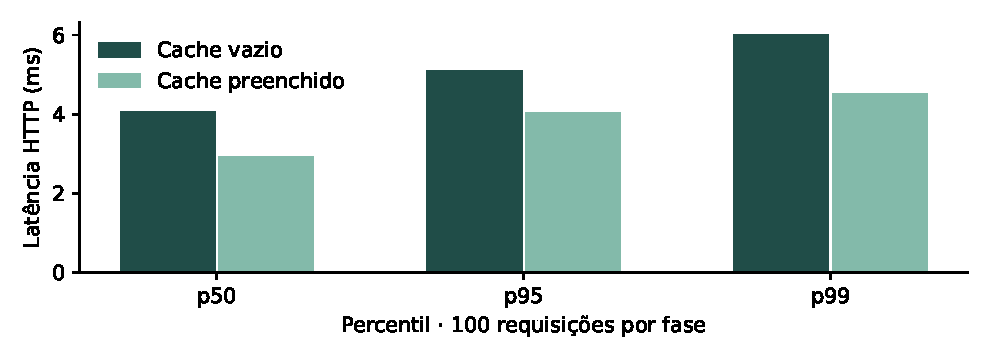
\includegraphics[width=.92\linewidth]{latencia.pdf}\\ Figura 1. Percentis de latência da API local.\end{center}
O p95 caiu de 5,11 ms para 4,04 ms na repetição. O p50 passou de 4,07 para 2,93 ms e o p99 de 6,02 para 4,53 ms. Com a palavra “ética”, quatro resultados e cache aquecido, o p95 foi 4,54 ms e o p99, 5,47 ms. O corpo maior altera o custo de serialização. Esses valores caracterizam apenas o ambiente e o corpus do ensaio.

Em 25 passagens pelos dois cadernos didáticos, a mediana de extração de seis itens foi 10,23 ms, aproximadamente 587 documentos/s. O intervalo inclui abertura dos PDFs, segmentação e validação. Exclui download, Kafka, atualização do índice e refresh. Para medir a vazão distribuída, o script vazao publica IDs inéditos e cronometra até a visibilidade do último ID pela API.

\section*{8.2. Resiliência e controle de acesso}
A demonstração exercitou autenticação local, consulta interdisciplinar, cache, carrinho e exportação. O estudante recebeu HTTP 403 em exportação e análises; o professor recebeu HTTP 200 e o gabarito na exportação. A validação das rotas foi executada com o mesmo código FastAPI usado pelo cluster. O adaptador local substitui LDAP, Redis e Elasticsearch nesse ensaio.

O teste distribuído previsto interrompe o consumidor, publica seis IDs inéditos, restaura o serviço e republica o lote. A condição de aprovação é encontrar os seis IDs e manter a cardinalidade após a repetição. O log registra o lag de cada partição como a diferença entre o próximo offset do broker e o offset processado mais um. Sem Docker disponível no ensaio, não foi possível declarar perda zero, lag observado ou hit rate do Redis.

\clearpage
\section*{9. Gargalos e lições}
O custo mais difícil de estimar está na curadoria de documentos heterogêneos. Reconhecer uma letra de gabarito é uma operação mais simples que separar duas alternativas intercaladas por uma imagem. Por isso, a validação por campo precisa ser complementada pela inspeção do item inteiro. A ferramenta de amostragem seleciona 50 IDs únicos com semente fixa e gera uma ficha com PDF, página, texto, alternativas, chave, mídia e metadados.

O consumidor usa refresh com espera antes da invalidação global do cache. Isso simplifica a leitura após escrita, mas pode reduzir a vazão quando cada registro aguarda o próximo refresh. Um teste de lote deve comparar documentos por segundo, latência de visibilidade e lag. A topologia de host único também limita a interpretação de resultados de disponibilidade.

\section*{10. Conclusão}
O protótipo permite seguir um item desde a página do caderno didático até sua seleção e exportação por professor. A busca por ética recuperou quatro itens em dois cursos, e o acesso direto de estudante à exportação foi bloqueado. A entrega do acervo completo exige conciliar o inventário oficial, auditar 50 questões integrais e executar a implantação segura com suas métricas. Os scripts e resultados brutos tornam explícito o ponto de partida para essa validação.

\section*{11. Divisão de tarefas e declaração de IA}
O trabalho está identificado em nome de Kaike Ferreira Alves. Não foram informados outros integrantes nem uma divisão efetivamente realizada. A organização técnica compreende curadoria documental, serviços de dados, API e segurança, e avaliação. A atribuição de participação individual deve corresponder ao trabalho efetivo de cada integrante.

O assistente ChatGPT da OpenAI apoiou a redação, geração de código, exemplos didáticos e organização dos ensaios. Não houve chamada a API de LLM na extração ou inferência multimodal. Custo adicional de inferência do pipeline: R$ 0. Não se aplica taxa de erro de modelo extrator; a avaliação do leitor determinístico e suas limitações constam na seção 8.

\section*{Referências}
[1] Inep. ENADE: provas e gabaritos por edição. \url{https://www.gov.br/inep/pt-br/areas-de-atuacao/avaliacao-e-exames-educacionais/enade/provas-e-gabaritos}\par
[2] Inep. Gabarito definitivo de Sistemas de Informação, 2021. \url{https://download.inep.gov.br/enade/provas_e_gabaritos/2021_GB_bacharelado_sistema_informacao.pdf}\par
[3] Inep. Gabarito definitivo de Análise e Desenvolvimento de Sistemas, 2021. \url{https://download.inep.gov.br/enade/provas_e_gabaritos/2021_GB_tecnologia_analise_desenvolvimento_sistemas.pdf}\par
[4] Elastic. Security settings in Elasticsearch: Kerberos realm. \url{https://www.elastic.co/guide/en/elasticsearch/reference/8.19/security-settings.html}\par\end{document}